%SOP Template 
% Version 02 Added revision date
% Version 03 Added TOC and acknowledgements
%           New SOP3_alpha.cls
% Version 04 Revised Set Up and included images

\documentclass[12pt]{../SOP3}\usepackage[]{graphicx}\usepackage[]{color}
%% maxwidth is the original width if it is less than linewidth
%% otherwise use linewidth (to make sure the graphics do not exceed the margin)
\makeatletter
\def\maxwidth{ %
  \ifdim\Gin@nat@width>\linewidth
    \linewidth
  \else
    \Gin@nat@width
  \fi
}
\makeatother

\definecolor{fgcolor}{rgb}{0.345, 0.345, 0.345}
\newcommand{\hlnum}[1]{\textcolor[rgb]{0.686,0.059,0.569}{#1}}%
\newcommand{\hlstr}[1]{\textcolor[rgb]{0.192,0.494,0.8}{#1}}%
\newcommand{\hlcom}[1]{\textcolor[rgb]{0.678,0.584,0.686}{\textit{#1}}}%
\newcommand{\hlopt}[1]{\textcolor[rgb]{0,0,0}{#1}}%
\newcommand{\hlstd}[1]{\textcolor[rgb]{0.345,0.345,0.345}{#1}}%
\newcommand{\hlkwa}[1]{\textcolor[rgb]{0.161,0.373,0.58}{\textbf{#1}}}%
\newcommand{\hlkwb}[1]{\textcolor[rgb]{0.69,0.353,0.396}{#1}}%
\newcommand{\hlkwc}[1]{\textcolor[rgb]{0.333,0.667,0.333}{#1}}%
\newcommand{\hlkwd}[1]{\textcolor[rgb]{0.737,0.353,0.396}{\textbf{#1}}}%
\let\hlipl\hlkwb

\usepackage{framed}
\makeatletter
\newenvironment{kframe}{%
 \def\at@end@of@kframe{}%
 \ifinner\ifhmode%
  \def\at@end@of@kframe{\end{minipage}}%
  \begin{minipage}{\columnwidth}%
 \fi\fi%
 \def\FrameCommand##1{\hskip\@totalleftmargin \hskip-\fboxsep
 \colorbox{shadecolor}{##1}\hskip-\fboxsep
     % There is no \\@totalrightmargin, so:
     \hskip-\linewidth \hskip-\@totalleftmargin \hskip\columnwidth}%
 \MakeFramed {\advance\hsize-\width
   \@totalleftmargin\z@ \linewidth\hsize
   \@setminipage}}%
 {\par\unskip\endMakeFramed%
 \at@end@of@kframe}
\makeatother

\definecolor{shadecolor}{rgb}{.97, .97, .97}
\definecolor{messagecolor}{rgb}{0, 0, 0}
\definecolor{warningcolor}{rgb}{1, 0, 1}
\definecolor{errorcolor}{rgb}{1, 0, 0}
\newenvironment{knitrout}{}{} % an empty environment to be redefined in TeX

\usepackage{alltt}

\usepackage[english]{babel}
\usepackage{blindtext}
%\usepackage{lipsum}

\usepackage{graphicx}

\title{Greenhouse Gas Measurements w/Picarro}
\date{5/4/2017}
\author{Isaac Medina and Allison Joseph}
\approved{Los Huertos}
\ReviseDate{\today}
\SOPno{38 v.03}
\IfFileExists{upquote.sty}{\usepackage{upquote}}{}
\begin{document}

\maketitle

\section{Scope and Application}

\NP Covers how to install Eosense soil gas flux chambers (PN: 10089) and connect them to multiplexer (PN: 10197) and a Picarro G2508 (Santa Clara, USA) gas analyzer.

\NP Orginally, this SOP was developed for greenhouse gas emissions from strawberry fields in NorCal. It has been been modified as new projects come on line that rely on these instruments. 

\section{Summary of Method}

\NP This SOP describes how to 1) set up the Picarro, Multiplexer, Dynamic Soil Chambers, and Vacuum Pump. 

\tableofcontents

\newpage

\section{Acknowledgements}

We thank the work of Isaac Medina, Neha Vaingankar, and Baily Lai who worked with the instrutment early on and developed early versions of the SOP. 

\section{Definitions}

\NP Picarro G2508 is the latest Picarro analyzer that measures N2O concentration along with CH4, CO2, NH3 and H2O. 

  
\NP EosAC soil flux chambers (Eosense Inc, Dartmouth, Canada) is coupled with
the eosMX-P multiplexer (Eosense Inc, Dartmouth, Canada). The eosMX multiplexer connects up to 12 eosAC chambers to the gas analyzer. 

\NP Recirculation pump (PN: A0702) provides the vacuum required for sample gas sequencing into and out of the Analyzer. 

\section{Biases and Interferences}

\NP Biases and interferences

\begin{itemize} 
\item Ambient temperature can prevent the analyzer from stabilizing properly.

\item Tapping high moisture gas samples can cause condensation damage to the instrument. To prevent such damage, a flow of clean, relatively dry gas should always be directed through the instrument for several minutes prior to shutdown. 

\end{itemize}

\NP Calibation Changes
\begin{itemize}

\item The analyzer’s calibration is intended to be done infrequently. It is only necessary to use three calibration standards to calibrate each gas or isotopic species (two points define the calibration line and a third intermediate point is used for verification).

\item When calibrating, the exact value of each calibration standards is not of particular importance as long as they span a representative range of values over which the analyzer will typically be operated. It is reasonable to use a concentration of zero for the low calibration value, for example. 
\item To perform a calibration or verification of calibration, the user simply introduces the first calibration standard into the analyzer for an interval long enough for the analyzer to yield a stable measurement of that sample. 
\item The stated concentration of the calibration sample (a permeation tube or calibrated gas bottle, for example) and the value the analyzer reads for that sample are recorded for each calibration standard used. 
\item These values can then be plotted, as shown below, in a spreadsheet, for example, to determine the linear relationship between the known calibration values and the analyzer’s reported values.

\begin{figure}
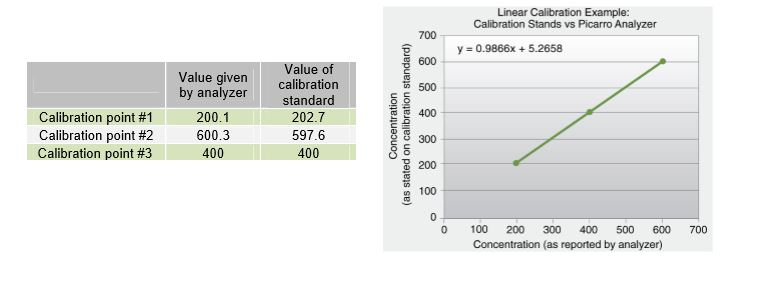
\includegraphics[width=400]{"/home/CAMPUS/aeja2017/SOPs/38_Picaro_GHG/graphics/calibration.jpg"}
\end{figure}


\item A linear best-fit equation can be calculated from the data. It is important to plot the analyzer’s reported concentration on the horizontal axis and the gas standards’ stated concentrations on the vertical axis.
\item The slope and intercept of the best-fit line through these points are the two values that are used to calibrate the analyzer. By determining what the linear relationship is between the known calibration values and the analyzer’s reported concentration values in this way, a calibration offset (slope and intercept) can be calculated so as to add a correction term to the analyzer’s factory or previous calibration. 
 
\section{Health and Safety}

\NP Describe the risk...


\subsection*{Safety and Personnnel Protective Equipment}


\section{Personnel \& Training Responsibilities}

Researchers training to use the Eosense chambers and Picarro analyzer include the following components: 



Researchers using this SOP should be trained for the following SOPs:

\begin{itemize}
  \item SOP03 Field Work
  \item SOP04 Electrical Power in the Field
\end{itemize}

Unanswered Picarro Questions

\NP Set up tool / Data Logger setup: what is difference between dry and regular and timed Data columns

\NP What is etalon temp (part of sensors in data source)

\NP We need an SOP for calibration, including parts to order

\NP Recommendations for car-mounting? Is okay to stack the multiplexer on top?

\NP Is there are way to turn on computer without turning on the gas analyzer and vacuum? 

\NP What files do we need to send to marc for him to reprocess them.

\NP N2O is very noisy. Is there a way to reduce the noise?

Picarro
Data Source/ sensors: allows you to see all sensor readings on picaro
controller: zoom in/out= right and left mouse click






Forunner Multiplexer Questions

\NP In the chamber data processor what does (L) or (E) mean in displaying fluxes for graphs?\ldots for example Flux CO2 (L) or Flux CO2 (E) 

\NP In options for measurements chart in the data processor what is dead band range and what is chamber offset? 

\NP Are we supposed to measure chamber offset for each of the chambers we set out? (distance between bottom of chamber and soil due to collar)


\section{Required Materials and Apparati}

\NP Picarro G2508 S/N 2143-JFAADS2048

\NP Eosense (Forerunner) Multiplexer S/N ??

\NP Chambers with Cables and Teflon Tubing (X meters in length)

\begin{table}
\caption{EosAC soil flux chambers (Eosense Inc, Dartmouth, Canada)}
\begin{tabular}{cc} \hline
Chamber S?N   & Filed ID \# (2015-16)  \\ \hline\hline
1001501       &         \\
1001502       &  5       \\
1001503       &  2       \\
1001504       &   3      \\
1001505       &   4      \\
1001506       &         \\
1001507       &  1       \\
1001508       &         \\
1001509       &         \\
1001510       &         \\
1001511       &         \\
1001512       &         \\ \hline
\end{tabular}
\end{table}


\NP In addition, we have identified the following customer support contacts:

\begin{itemize}
  \item Picarro Tech support: Melissa, 408-962-3978
  \item Scott (408-962-3987)
  \item Karrin Alstad Applications --- get calibration stuff from her. 408-962-3991
\end{itemize}

\NP Eosense (East Coast Time Zone)

\begin{itemize}
  \item Customer support: 888.352.8313 (toll-free)
  \item Email: support@eosense.com
\end{itemize}

\section{Reagents and Standards}

\NP Standards..\cite{StandardMethods2012}.

\NP Driorite


\section{Estimated Time}

\NP Setting up the Picarro can take between 1-1 1/2 hours depending on your experience. Depending on the ambient temperature, the Picarro can take ~30 minutes to reach operating temperatures. To be effecient, start the Picarro as soon as possible.

\section{Sampling Design}

\NP The cable and gas tubing is XX meter.

\NP If the generator is used, place the it downwind at a minium of 100 feet.

\section{Set Up}

\NP Connect pump to Analyzer VACUUM port using the convoluted metal hose. Hand tighten and use wrench to seal connection.

\NP 
\begin{figure}[h]
\includegraphics[width=.5\textwidth]{"/home/CAMPUS/aeja2017/SOPs/38_Picaro_GHG/graphics/pump_multiplexer"}
\caption{Pump to Multiplexer}
\end{figure}


\NP Connect multiplexer to Picarro through USB ports on Picarro (does not matter which port used)

\NP Connect monitor, mouse, and keyboard to Picarro via the remaining USB ports (note: there are two extra USB ports on the front of the Picarro)

\NP Connect blue monitor plug to Picarro and monitor power plug to outlet.

\NP Ensure all machines are in the off position (the circle signifies off position)

\NP Connect power plugs for CRDS, multiplexer, and pump

\NP Connect pump to multiplexer
\begin{itemize}
\item Connect control and data ports on the back of the pump to the Picarro ensuring white triangles are facing up on the back of the pump
\item Insert other cable end of these connections into any USB port on the Picarro
\end{itemize}

\begin{figure}
\includegraphics[width=400]{"/home/CAMPUS/aeja2017/SOPs/38_Picaro_GHG/graphics/whitetriangleusb"}
\end{figure}

\NP Connect clear tubes to an inlet port on the pump, connect other end to the inlet on the front of the multiplexer
\begin{itemize}
\item Inlet on multiplexer on right (labeled)
\item Inlet on vacuum (on left -- clear tube)
\end{itemize}



\NP Repeat process for the outlet tubes
\begin{itemize}
\item Outlet on Picarro
\item Outlet on vacuum (on right -- silver tube)
\end{itemize}

\NP Attach clear tube inlet of Picarro to labeled outlet on multiplexer

\NP Attach one end of power/data cable to the COMM port in the pump and the other end to the matching COMM port on the multiplexer

\begin{figure}
\includegraphics[width=300]{"/home/CAMPUS/aeja2017/SOPs/38_Picaro_GHG/graphics/COMM"}
\end{figure}

\NP Power on pump and Picarro **Never turn off pump when Picarro is on**

\subsection*{Selection the Proper Location for Instruments}

\NP Machine serves as base location.
\NP Use random number generator to determine location for each of the chambers.

\subsection*{Installing Chamber Rings}

\NP This will vary based on the design of your experiment. 

\subsection*{Picarro Start up Procedure}

\NP Connect to power supply

\NP Make sure all instruments are in the off position and turn on power strip

\NP Turn-on recirculation pump (apparently there is no wait time)

\NP Pump must be turned on before starting G2508 analzyer. Never disconnect vacuum will analyzer is running.

\NP Keep ambient temperature below 35\degree C

\NP Switch on Picarro  -- Boot up sequence initializes CRDS software and analyzer

\NP Switch on Multiplexer. Warming up for 30 minutes -- warning error until everything needs to be heated.

\subsection*{Place Chambers on Rings}

\NP Place chambers onto bases, pressing ring down to get a good seal. Try to avoid disturbing the chamber after it has been installed. 

\NP Connect all hoses while Picarro is warming up. --place tubing along the bed (dont let them get into the furrow)

\NP After all chambers have opened up, do a second check for foliage that might get in the way

\subsection*{Data Collection (when alarm is green)}

\NP Check Picarro Conditions

\NP Ambient should be below 35\degree C. (DAS -- if DAS goes up to 45\degree, should be turned off or cooled -- Use fan to cool air around the Picarro.
                               
\NP Check for typical atmospheric concentrations:
                                 
\begin{itemize}
\item N2O ~ 0.3 ppm
\item CH4 ~ 2.4 ppm
\item C2O ~ 300-600 ppm
\item NH3?
\item H2O ~ 1-5\%
\end{itemize}
                               
\subsection*{Start Multiplexer Software}

\NP FP-Monitor??
                               
\NP Uncheck default cycle
                               
\NP Load cycle in user folder. The following cycles are avaialble 

\begin{description}
  \item[straw 5 chamber ??? names?]
  \item[Full 12]
  \item[Full 12 minus \#4]
\end{description}
()
                               
\NP When Picarro G2508 is warm, initiate cycle -- "start cycle"??
                               
\NP Check chambers to ensure good seals
                               
\NP Check fuel every two hours, top off each time -- be careful to avoid spilling. Be sure to release pressure before putting nozzle into filler throat. Open valve for gas when nozzle is inserted nearly into generator filler throat. Press green button for 3-5 sec intervals, checking between filling to determine if the gas at at or near the red line.
                               Try to get at least 3 cycles minimum . ideal is 2 cycles before irrigation, 2 cycles during irrigation and 2 cycles after. 
                               
\subsection*{Shut-Down Procedure}
                               
\NP After at least two cycles after irrigation, begin retrieving chambers after each one has completed measurements (starting at 1 usually).
                               
\NP Cap all sets of tubes with glove and tape.
                               
\NP Carefully coil each set of tubes and wires to limit twisting and scratching of teflon. Zip/velcro together and stack in order 1-5 on the ground. 
                               
\NP Remove chambers from sampling location
                               
\NP Separate based from chamber and repackage them into boxes.
                               
\NP When final chamber measurement has been completed, "end" ? sampling cycle
                               
\NP Connect spare chamber to channel X and refresh chamber... 
                               
\NP select "Desciccate" method and run dry air through Picarro for 10 minutes.
                               
\NP shut down.
                               
\NP Shut down Picarro --- Select option for moving instrument.
                               
\NP After Picarro shuts down, manually switch off:

\begin{enumerate}
  \item Multiplexer
  \item Picarro
  \item Vacuum Pump
  \item Power Strip
\end{enumerate}
                               
\section{Data Analysis and Calculations}
\NP 
\section{QC/QA Criteria}


\section{Trouble Shooting}
How to read data from Picarro (must be emailed)
The Chamber Data Processor program is expecting to find all of the relevant 

%"FRMonitor_0000.log, FRMonitor_0001.log..." 
files in its own folder. You can freely move these out between sites, but as they contain information about the chamber sequencing, when you are processing a certain date range, you will need to have to correct FRMonitor logs present (the program will start its search with log 0000 and go until it cannot find the next in the sequence). 
The path for raw analyzer data should always be the same, and should look like:  
%C:/UserData/DataLog_Forerunner. 

You can set this from the Data menu in the Chamber Data Processor (Data-> Analyzer Data Path).

Days with unexpected data:  These days (159 and 175 or June 8th and June 24th) appear to contain valid chamber measurements. The Julian Day metric is pulled directly from the raw analyzer data and there don't appear to be any cases where a measurement got moved from the proper day. I would check to see if the system and/or local time on the analyzer have been changed, as this could potentially cause problems. You could also compare the processed measurements against your field notes to see if there is an obvious time period with missing data that seems to match with these days.

Days that should have more data: I noticed several errors in the FRMonitor logs that you uploaded. I've fixed these files and attached them to this email. Back up the older versions and try using these instead: I noticed several additional measurements appear once I had updated them. As for where these errors came from, the log files suggest that, at some points at least, chambers were disconnected from the Multiplexer while it was actively running a measurement cycle? If so, I would strongly advise against this, as it can cause the Chamber Data Processor to overlook measurements (especially if the chamber was closed when it was removed). Also, are you using the 1.6.0 or 1.6.2 version of the FRMonitor software? Make sure to use the newer version to schedule measurements.


Days where some chambers are missing: I saw several days where Chambers 1 and/or 2 do not appear to be sending any data. This indicates either a communication issue between the Multiplexer and Analyzer, or that the chambers were not connected during this time period. Has the FRMonitor software been recognizing all of the connected chambers on start-up?  If not, then they will not record data (even if they open and close). The System Info button will show you a break down of chamber-specific events, including successfully logged measurements and communication problems. Disconnecting and reconnecting chambers during a measurement cycle can also cause these errors.




\section{References}

\bibliography{../SOP.bib}

\NP APHA, AWWA. WEF. (2012) Standard Methods for examination of water and wastewater. 22nd American Public Health Association (Eds.). Washington. 1360 pp. (2014).

\end{document}
